
\chapter{ROS与PX4介绍}\label{introduction}

\section{ROS介绍}
本文这一节主要介绍用于描述飞机姿态位置的坐标系与坐标系之间的转换,用来推导四旋翼飞控建模过程中需要用的旋转矩阵与转换方程。飞机的姿态描述需要利用各种坐标系表示的原因如下:

\begin{enumerate}
	\item 空气动力学的力和力矩是在机体坐标系下表示的。
	\item 牛顿运动方程利用四元数法来表示,需要指明相关的坐标系。
	\item 在机体坐标系下,飞机传感器读取飞机姿态参数信息,比如加速度;相反,飞机上GPS系统读取的飞机位置姿态参数需要在惯性坐标系下(即地面坐标系)。
	\item 大多数情况下,需要在惯性坐标系下,对飞机的飞行轨迹进行描述。另外,地图所采用的位置坐标也是在惯性坐标系下表示的。
\end{enumerate}

要想完成一个坐标系到另一个坐标系之间的转换,需要完成两个步骤,一个是旋转,另一个是转换。在本章的\ref{2.1.1}节部分用来描述坐标旋转矩阵和旋转矩阵应用于坐标系变化;在本章的\ref{2.1.2}节部分用来介绍在四旋翼无人机系统下所采用的特定坐标系,推导四旋翼旋转矩阵表达式;在本章的\ref{2.1.3}节部分用来推导坐标系转换过程中转换关系,即Corlios方程。最终,推导完成坐标系转换过程的两个步骤:旋转和转换。


\subsection{ROS的消息机制} \label{2.1.1}

\begin{figure}[!ht]
\centering
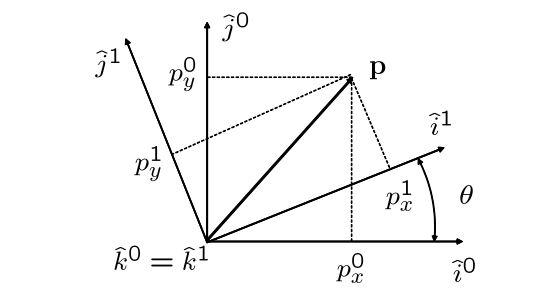
\includegraphics[width=0.6\textwidth]{f2.jpg}
\caption{坐标系二维旋转} 
\label{fig2}
\end{figure}

如图\ref{fig2}所示,向量{\bf{p}}即在坐标系$\mathop R\nolimits^0$下同时还在坐标系$\mathop R\nolimits^1$下,$\mathop R\nolimits^0$坐标系与$\mathop R\nolimits^1$坐标系的坐标原点相同,故向量{\bf{p}}从坐标系$\mathop R\nolimits^0$ 到坐标系$\mathop R\nolimits^1 $的旋转,属于二维空间的旋转。在坐标系$\mathop R\nolimits^0$下,单位向量用$\left( {{{\hat i}^0},{{\hat j}^0},{{\hat k}^0}} \right)$表示,在坐标系$\mathop R\nolimits^1 $下,单位向量用$\left( {{{\hat i}^1},{{\hat j}^1},{{\hat k}^1}} \right)$表示。在坐标系$\mathop R\nolimits^0$下,向量{\bf{p}}可以表示为:
%
\begin{equation}
\mathbf{p} = p_{x}^{0} \hat{i}^0 + p_{y}^{0} \hat{j}^0 + p_{z}^{0} \hat{k}^0
\end{equation}

同样,在坐标系系$\mathop R\nolimits^1 $下,向量{\bf{p}}可以表示为:
%
\begin{equation}
\mathbf{p} = p_{x}^{1} \hat{i}^1 + p_{y}^{1} \hat{j}^1 + p_{z}^{1} \hat{k}^1
\end{equation}

联立上面两式,可以得到如下的关系:
%
\begin{equation}
p_{x}^{1} \hat{i}^1 + p_{y}^{1} \hat{j}^1 + p_{z}^{1} \hat{k}^1 = p_{x}^{1} \hat{i}^1 + p_{y}^{1} \hat{j}^1 + p_{z}^{1} \hat{k}^1
\end{equation}



\subsection{gazebo仿真} \label{2.1.2}

在四旋翼飞行控制时,需要实现不同坐标系之间的转换,下面介绍常用的坐标系。

\subsubsection{惯性坐标系$\mathop R\nolimits^i $}

\begin{figure}[!ht]
\centering
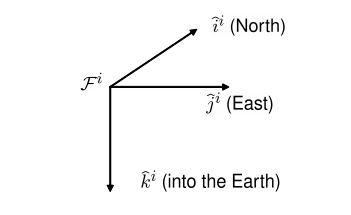
\includegraphics[width=0.4\textwidth]{f5.jpg}
\caption{惯性坐标系}
\label{fig4}
\end{figure}

惯性坐标系是指坐标原点位于地心,如图\ref{fig4}所示,向量$\hat i$指向北,向量$\hat j$指向东,向量$\hat k$指向地心。

\subsubsection{速度坐标系$\mathop R\nolimits^\nu$}

\begin{figure}[!ht]
\centering
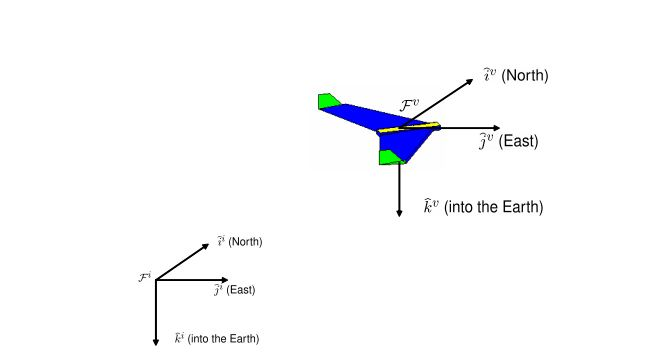
\includegraphics[width=0.9\textwidth]{f6.jpg}
\caption{速度坐标系}
\label{fig5}
\end{figure}



在这一节,本文打算推导Coriolis数学关系式为后面飞控动力学关系作铺垫,Coriolis公式在坐标系变换过程中,起到非常重要的作用。假设,我们有两个坐标系,机体坐标系$\mathop R\nolimits^b $和惯性坐标系$\mathop R\nolimits^i $,如图\ref{cfig9} 所示,向量${\bf{p}}$相对坐标系$\mathop R\nolimits^i $的运动,可以分解为两个运动,即:有向量${\bf{p}}$ 随着机体坐标系$\mathop R\nolimits^b $的平动,和向量${\bf{p}}$相对$\mathop R\nolimits^i $ 坐标系转动。

\begin{figure}[!ht]
\centering
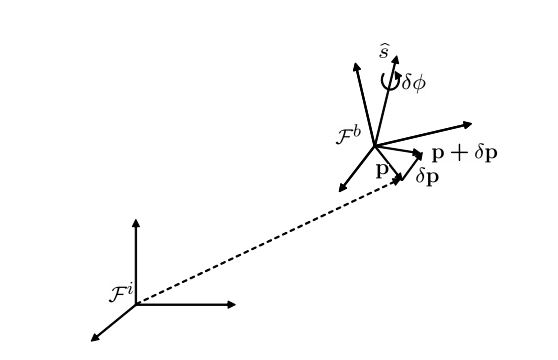
\includegraphics[width=0.6\textwidth]{f10.jpg}
\caption{Coriolis公式推导图}
\label{fig9}
\end{figure}



\section{PX4 AutoPilot}
本文将飞行摇杆(Joystick)数据读取作为四旋翼飞控模型的输入,Joystick数据的数据主要是四旋翼的姿态角(滚转角,偏航角,俯仰角)和四旋翼的推力。因此,本文通过C++编程,实现飞行摇杆数据的输入。由如下代码所示:

\begin{lstlisting}[language={[ANSI]C++}]
class HAL_JoyStick: public ZY::Thread {
public:
    HAL_JoyStick(){
        m_devID = -1;
    }
    HAL_JoyStick(int dev) {
        m_devID=dev;
    }
    virtual ~HAL_JoyStick() {}
    int open(int devID);
    void run();
    int close(void);
    int read(JS_Val *jsv)
    {
        data_mutex.lock();
        *jsv= m_JSVal;
        m_JSVal.dataUpdated = 0;
        data_mutex.unlock();
        return 0;
    }
public:
    int         m_devType;
    int         m_devID;
    int         m_devFD;
    char        number_of_axes;
    char        number_of_btns;
protected:
    ZY::Mutex   data_mutex;
    JS_Val      m_JSVal;
}
\end{lstlisting}

\subsection{FailSafe机制} \label{2.2.1}
\subsection{EKF与飞行模式} \label{2.2.2}
\subsection{联合MAVROS的Offboard模式} \label{2.2.3}



